\clearpage
\chapter{Matlab Problem 3.2: Information vs. Energy}

Zur Berechnung der Ausgangswerte des Systems wurde das System mit dem vorgegebenen Quantizer implementiert (siehe Listings) und f�r $10^6$ Samples mit 1 bis 5 Bit Simulationen durchgef�hrt. Der Quantisierer f�hrt teilt dabei den Eingangsbereich in eine der Anzahl an Bit entsprechenden Anzahl Stufen und rundet das Eingangssignal auf die n�chstliegende Stufe.

Mit der vorgegebenen Funktion \texttt{CondEntropy} wurden die bedingten Entropien berechnet, welche dem Informationsgehalt eines Wertes entspricht, wenn die vorherigen Werte bekannt sind.

Darstellungen \ref{fig:3_2_h_N0}, \ref{fig:3_2_h_N1} und \ref{fig:3_2_h_N2} stellen die bedingten Entropien bei unterschiedlichen $N$ dar.

Bei $N=0$ (Abb.~\ref{fig:3_2_h_N0}) sinkt die Entropie nach dem ersten Zeichen schnell, und danach langsamer. F�hrt man \emph{Linear Prediction} ein mit $N=1$ (Abb.~\ref{fig:3_2_h_N1}), so bleibt die Entropie weitgehend erhalten und sinkt nur langsam, der Informationsgehalt der �bertragenen Werte bleibt also h�her. Erh�ht man $N$ auf $2$ (Abb.~\ref{fig:3_2_h_N2}), so beginnt die Entropie wieder zu sinken, und zwar sogar schneller als im Fall $N=0$.

\begin{figure}[h!]
  \centering
  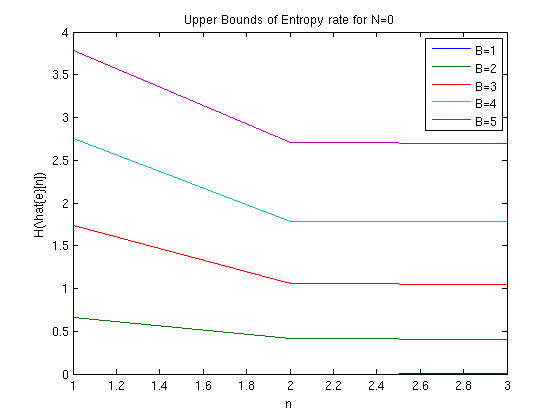
\includegraphics[width=0.7\textwidth]{./plots/3_2_h_N0.png}
  % 3_3_c_freqresponse.png: 560x420 pixel, 90dpi, 15.81x11.85 cm, bb=0 0 448 336
  \caption{Entropie f�r $N=0$}
  \label{fig:3_2_h_N0}
\end{figure}

\begin{figure}[h!]
  \centering
  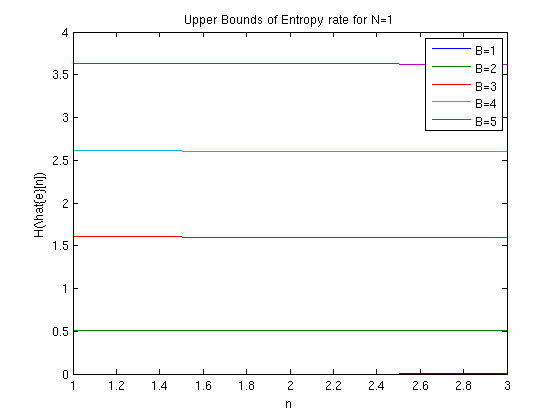
\includegraphics[width=0.7\textwidth]{./plots/3_2_h_N1.png}
  % 3_3_c_freqresponse.png: 560x420 pixel, 90dpi, 15.81x11.85 cm, bb=0 0 448 336
  \caption{Entropie f�r $N=1$}
  \label{fig:3_2_h_N1}
\end{figure}

\begin{figure}[h!]
  \centering
  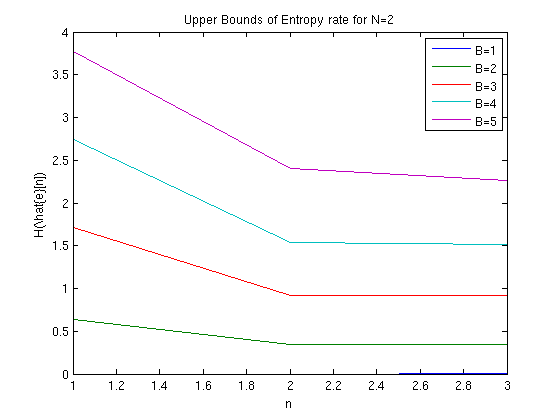
\includegraphics[width=0.7\textwidth]{./plots/3_2_h_N2.png}
  % 3_3_c_freqresponse.png: 560x420 pixel, 90dpi, 15.81x11.85 cm, bb=0 0 448 336
  \caption{Entropie f�r $N=2$}
  \label{fig:3_2_h_N2}
\end{figure}
